\chapter{Przygotowanie środowiska - automatyzacja}

Rozpoznanie numeru autobusu, ze względu na niewielką moc obliczeniową
urządzeń mobilnych, wymagało zastosowania algorytmu składającego się
z~co najmniej kilku kroków. Kolejne stopnie kaskady uszeregowane były
w~taki sposób, aby operując na dużych zbiorach danych - np.: pełne 
klatki z~kamery w~wysokich rozdzielczościach - używać algorytmów o~możliwie
najniższej złożoności obliczeniowej celem zawężenia pola poszukiwań.
Postępująca segmentacja obrazu miała umożliwić rozpoznanie
numeru autobusu w~czasie rzeczywistym, nie zależnie od klasy urządzenia.

Biorąc pod uwagę powyższe wymagania pierwszym krokiem
algorytmu była segmentacja obrazu poprzez wykorzystanie kaskadowego
detektora cech HAAR-a, LBP lub HOG.
Ze względu na różnice pomiędzy tymi detektorami pierwszym
doświadczeniem wykonanym na potrzeby tego opracowania było porównanie
ich wydajności i~dokładności. 

Sam proces uczenia detektorów był przedsięwzięciem bardzo żmudnym.
Dodatkowo wymagał dużych zbiorów danych uczących oraz zbioru testowego.
W~następnych podrozdziałach przedstawione zostały narzędzia, których
zadaniem miała być maksymalna automatyzacja i~optymalizacja procesu uczenia
oraz weryfikacji zarówno skuteczności jak i~wydajności uzyskanych wersji
detektorów.

Oczywiście w~dalszych podrozdziałach opisano kolejne robocze
kroki algorytmu, a~także narzędzia służące w~ich przygotowaniu oraz 
weryfikacji.

Celem tego rozdziału było więc udokumentowanie prób przeprowadzonych
na drodze do osiągnięcia jak najbardziej zoptymalizowanego 
i~zautomatyzowanego procesu przygotowywania oraz testowania detektorów,
a~także innych elementów docelowego systemu.

\section{Wspomaganie pobierania filmów z serwisu YouTube}

Pewnego rodzaju rozgrzewką było przygotowanie wtyczki do przeglądarki 
Firefox ułatwiającej pobieranie i wstępne katalogowanie filmów
udostępnianych za pośrednictwem serwisu YouTube.

Założenia oraz oczekiwania funkcjonalne wobec omawianego narzędzia były 
następujące:

\begin{enumerate}
    \item Wizualizacja stanu w~jakim znajduje się oglądany film - 
        możliwe są dwa stany:
    \begin{itemize}
        \item co najmniej jedna wersja filmu została już pobrana,
        \item film nie został pobrany w~żadnej wersji.
    \end{itemize}
    \item Możliwość pobrania wybranej wersji filmu w~odległości maksymalnie
        dwuch kliknięć licząc od poziomu przeglądania filmów w~serwisie,
    \item Tworzenie pliku CSV (\textit{ang. Comma Separated Value})
        z~danymi pobranych filmów, celem identyfikacji już pobranych
        pozycji. Plik powinien być tak skonstruowany aby można go było
        również wykorzystać do odtworzenia bazy filmów na dysku. W~razie
        awarii lub chęci przeprowadzenia całego procesu uczenia od
        początku.
\end{enumerate}

\subsection{Pierwsza wersja wtyczki - prezentacja stanu oglądanego filmu}

Przedstawienie stanu aktualnie oglądanego filmu odbywa się poprzez
kolor dodatkowej ikony wkomponowanej w~lewe pionowe menu, zaraz obok
wyświetlanego filmu.

\begin{figure}[h!]
    \caption{Przycisk rozwijanego menu, oraz wskaźnik stanu}
    \centering
    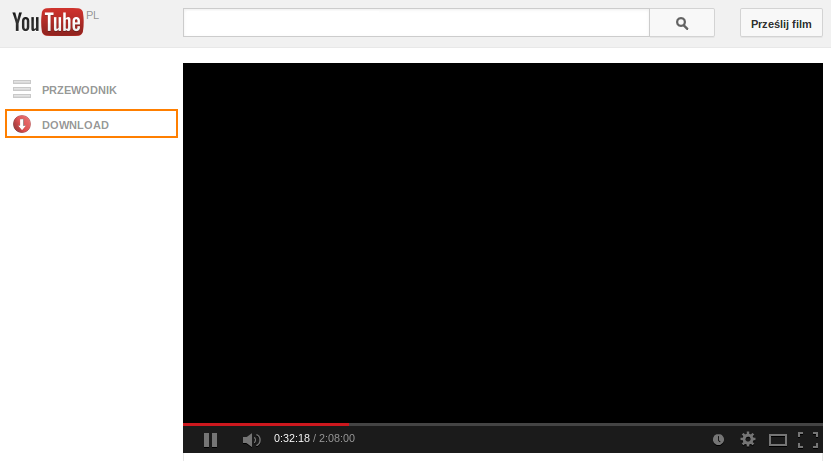
\includegraphics[width=0.9\textwidth]{img/env_yt_dwn_indicator}
\end{figure}

Kolor czerwony wskazuje, że oglądany film nie został jeszcze pobrany.
Ikona z~pustą strzałką w~środku w~kolorze zielonym sygnalizuje obecność
oglądanej pozycji w~wyżej wymienionym pliku rozdzielanym przecinkami
(pkt. 3).

Postępy w~pracach nad pierwszą wersją wtyczki doprowadziły do wypełnienia
założeń funkcjonalnych przez ostatnią wersję programu. Koncepcja wkomponowania
menu w~treść strony, oraz funkcjonalność pobierania filmów okazały się
na tyle problematyczne i~trudno zarządzalne, że powstała druga wersja programu
o~znacznie ograniczonej funkcjonalności.

\subsection{Druga wersja wtyczki - omówienie funkcjonalności}

Funkcjonalność drugiej wersji programu została ograniczona do minimum. Faktycznie
ograniczała się ona do oznaczania wybranego filmu wraz z~jego wersją, oraz
eksportu tak utworzonych wpisów do pliku - id filmu oraz numer identyfikacyjny wersji.

Przepływ sterowania dla drugiej wersji programu został przedstawiony na poniższym
diagramie. Funkcja implementująca pokazany algorytm była wywoływana za każdym razem
gdy zmieni się wartość url-a w~aktywnej karcie przeglądarki lub kliknięty został
któryś z~przycisków w stanach ,,żółtym'' lub ,,zielonym''.

\begin{figure}[h!]
    \caption{Algorytm aktualizacji stanu wtyczki w wersji drugiej}
    \centering
    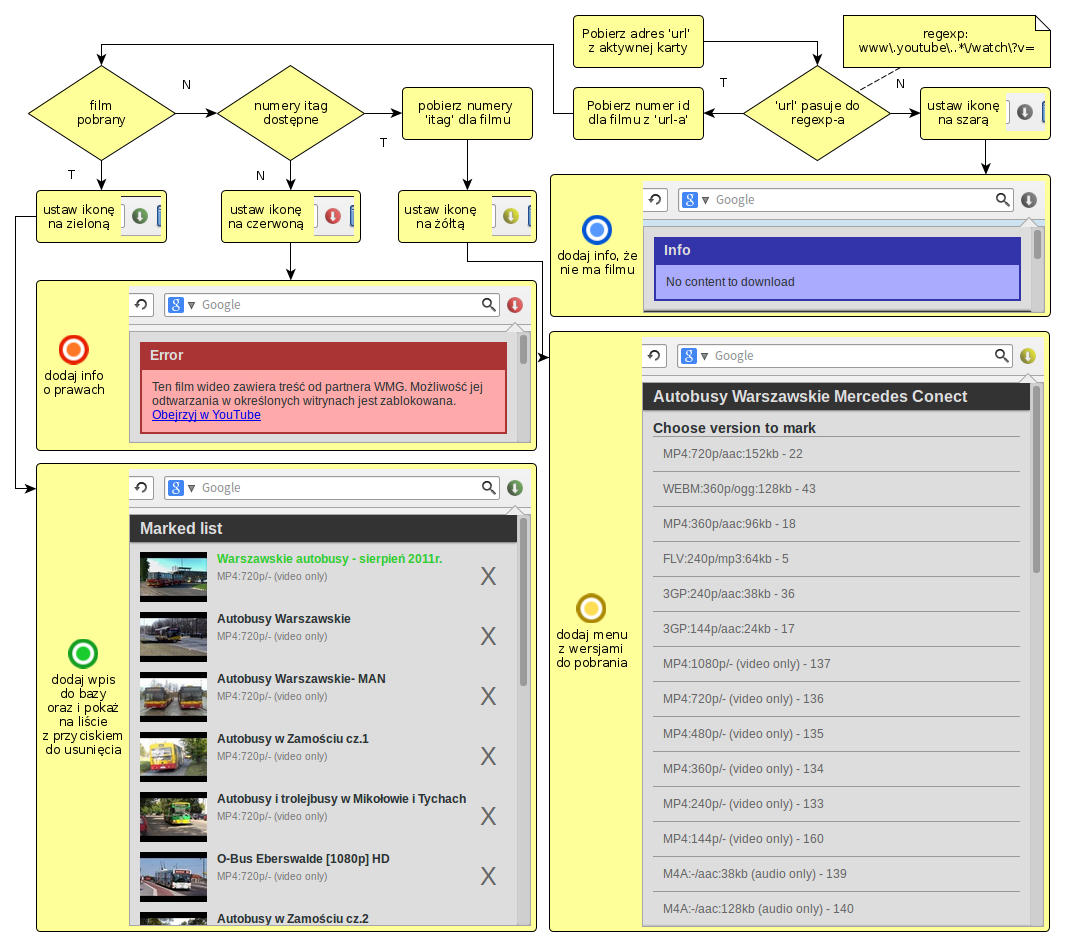
\includegraphics[width=0.9\textwidth]{img/env_yt_marker}
\end{figure}

Niestety pierwszy program ,,pomocniczy'' okazał się narzędziem nie adekwatnym
(zbyt skomplikowanym i~pracochłonnym) do postawionego mu zadania. Okazało się, że
filmów zawierających fronty autobusów jest znacznie mniej niż mogło by się wydawać.

Po znalezieniu 14 pozycji zawartość serwisu (w~kontekście frontów
autobusów) nagle się
wyczerpała. Ostatecznie wielotygodniowe (dokładnie dwu) prace nad wtyczką do programu 
Firefox zaowocowały bazą czternastu pozycji w~formie pliku CSV zawierającego dwie
kolumny:

\begin{itemize}
    \item id filmu, np.: 75Dz6s7S-Tg;
    \item itag reprezentujący wybraną wersję, np.: 136
\end{itemize}

W~naszym przypadku wszystkie filmy zostały ,,oznaczone'' w~wersji 136, czyli
zawierającej tylko obraz, oraz będącej w~rozdzielczośći HD (720p).

Ostatecznie owoc pracy przedstawiony jest poniżej.

\lstinputlisting{../data/description_files/marked_for_download/yt_marked_01.csv}

Co niestety o~wiele szybciej, prościej, wydajniej, taniej i~krótko mówiąc lepiej można
by wykonać bez implementowania żadnych narzędzi. Jedyne co pozostało to zdobyta wiedza
na temat: javascript, css, html, firefox: xul, addon-sdk, cfx. 

Kolejne narzędzia ,,pomocnicze'' implementowane były z~większą 
ostrożnością i~po
dłuższym przeanalizowaniu zagadnienia poddawanego automatyzacji.

\section{Tworzenie zbioru wejściowego do narzędzia train\_cascade}

Mając plik z~identyfikatorami filmów na serwisie YouTube wszystkie duże objętościowo
dane potrzebne przy tworzeniu wsadu od narzędzia uczącego można było zostawić
w~ich pierwotnym położeniu. Tworząc narzędzie wspomagające oznaczanie frontów
wzbogacono je o~możliwość odtworzenia osiągniętego stanu w~oparciu o~pliki konfiguracyjne.
Dodana funkcjonalność i~systematyczne wypychanie danych do zewnętrznego repozytorium
umożliwiły niezakłóconą kontynuację prac po awarii i~utracie lokalnej kopii.

Interfejsem narzędzia odpowiedzialnego za przygotowanie danych uczących był skrypt
napisany w~języku python:

\lstinputlisting{data/autocascader.txt}

\subsubsection{Odtwarzanie środowiska po awarii}

Pierwszym krokiem było pobranie plików wideo. W~tym celu należało wywołać skrypt
z~parametrem \verb|-d|.

Po drobnych poprawkach (utworzeniu katalogu na pobrane pliki, którego nie było
w~repozytorium) i~pobraniu wymaganych zależności proces poprawnie pobrał
11 (jedenaście) zdefiniowanych w~pliku konfiguracyjnym pozycji.

Ostatecznie wywołanie skryptu z~parametrem \verb|-e| poprawnie wyłuskało klatki
z~pobranych plików, które zostały zapisane w~postaci obrazów w~katalogach
odpowiadających ich przeznaczeniu:

\begin{itemize}
\item front - pliki reprezentujące generyczne fronty autobusów,
\item solaris - pliki reprezentujące fronty autobusów Solaris (dla porównania),
\item background - pliki tła - nie zawierające wystąpień żadnych frontów.
\end{itemize}


\section{Pozostałe narzędzia}

W~miarę jak prace nad algorytmem i~implementacją postępowały, powstawały
coraz to nowe narzędzia pomocnicze, których mnogość i~prostota nie
pozwalały na zamieszczenie ich szczegółowego opisu. 

Problem którego nie udało się zautomatyzować to weryfikacja skuteczności
całego algorytmu oraz poszczególnych jego części składowych. Pierwszą
próbą weryfikacji skuteczności było prymitywne porównywanie współrzędnych
wykrytego fragmentu z~tak zwaną \textit{,,ground truth''} - oznaczonymi
wystąpieniami szukanych obiektów, wykonanymi na potrzeby uczenia 
detektorów. 
Przyjęty margines błędu - (+/-) 1/4 wysokości i~szerokości - skutkował dość
wysokimi uzyskanymi współczynnikami skuteczności. Podejście to okazało
się jednak zupełnie nieadekwatne do postawionego zadania.

\begin{figure}[h!]
    \caption{Błędne założenia przy implementacji narzędzi do
    weryfikacji skuteczności}
    \centering
    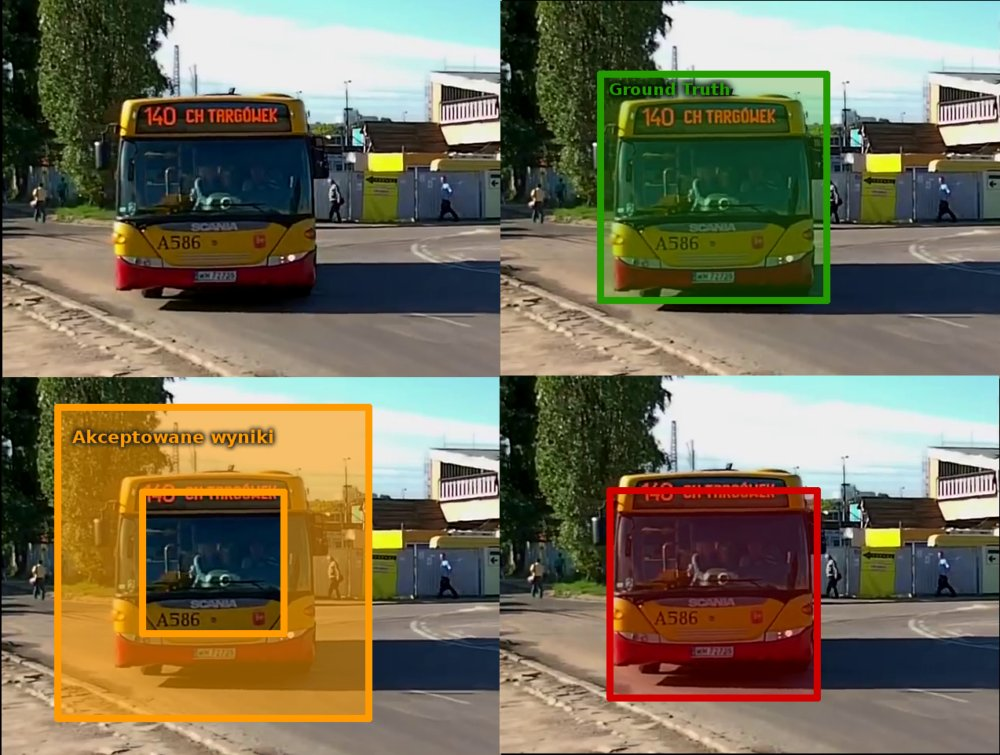
\includegraphics[width=0.9\textwidth]{img/env_benchmark_fail_1}
\end{figure}

Zastosowana metoda przemycała (jako pozytywne) wyniki zupełnie
bezwartościowe z~punktu widzenia postawionego problemu, którym było
odczytanie numeru nadjeżdżającego autobusu. Na rysunku 
powyżej jest przykład - zaznaczony na czerwono - wykrycia zaliczonego
jako pozytywne, które uniemożliwia odczytanie numeru z~powodu obcięcia
jego górnej części.

Dodatkowym utrudnieniem była ostateczna forma zbioru wykorzystanego 
do uczenia detektorów. Pierwsze podejście do problemu nauki 
detektorów wykorzystywało pełne klatki zawierające interesujący obiekt
plus plik tekstowy wskazujący współrzędne czworokąta okalającego.
Ogólny odsetek wykryć na takim zbiorze był zadowalający. Niestety
ostatecznie zrezygnowano z~przechowywania pełnych klatek na rzecz
wycinków reprezentujących wyłącznie instancje szukanych obiektów.
Było to spowodowane ograniczeniem przestrzeni dyskowej. Zbiór pełnych
klatek zajmował 32 GB, gdzie te same dane - fronty autobusów - po
przycięciu zajmowały nieco ponad 2 GB przestrzeni dyskowej.

Niestety taka forma przechowywania danych spowodowała sfałszowanie 
wyników automatycznego weryfikatora skuteczności. Co było jedną
z~wielu przyczyn całkowitego zaniechania syntetycznych testów skuteczności.

W~momencie pisania tego tekstu ukończony był już pierwszy
działający prototyp kompletnej aplikacji na urządzeniu mobilnym
z~systemem android. Niestety wszystkie testy wykonywane były
w~sposób empiryczny, manualny i~mocno subiektywny. Co za tym idzie,
liczba próbek - wykorzystanych danych testowych - była bardzo niewielkich
rozmiarów.
